\begin{figure}[htbp]
\centering
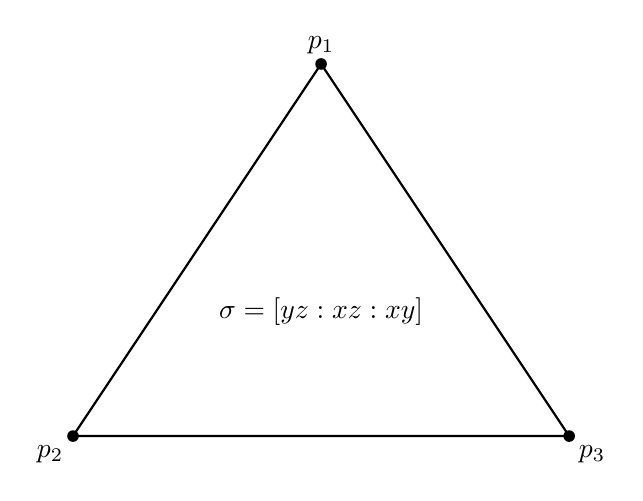
\begin{tikzpicture}[scale=1.05]
\coordinate (p1) at (0,3); \coordinate (p2) at (-3,-1.5); \coordinate (p3) at (3,-1.5);
\draw[thick] (p1)--(p2)--(p3)--cycle;
\fill (p1) circle (2pt) node[above] {$p_1$};
\fill (p2) circle (2pt) node[below left] {$p_2$};
\fill (p3) circle (2pt) node[below right] {$p_3$};
\node at (0,0) {$\sigma=[yz:xz:xy]$};
\end{tikzpicture}
\caption{The base triangle of the standard quadratic transformation.}
\label{fig:vi44-base-triangle}
\end{figure}
